\renewcommand{\vec}[1]{\textbf{#1}}

\chapter{Experimental Results}
\label{cha:experimental_results}

\section{2D Density Esitmation}

To test the simple model from Section \ref{sec:simple_pc} with the discussed algorithms, so Expectation Maximization (EM), 
Gradient Descent (GD), Score Matching (SM) and Sliced Score Matching (SSM) from subsections \ref{sec:gmm_em} to \ref{sec:gmm_ssm}, we used some 
two dimensional data to perform density estimation. 

Samples from the three datasets we used can be seen in Figure \ref{fig:2d_datasets}. \\

\vspace{10pt}
\begin{figure}[H]
    \centering
    \begin{subfigure}[b]{0.4\textwidth} 
        \centering
        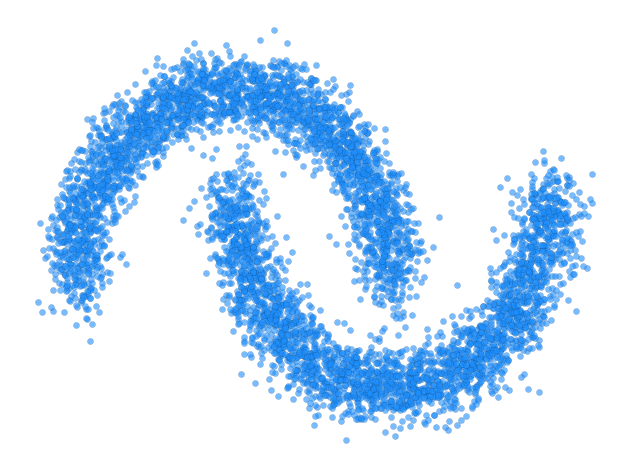
\includegraphics[width=\textwidth]{figures/halfmoons.png}
        \caption{halfmoons}
    \end{subfigure}
    \hfill
    \begin{subfigure}[b]{0.4\textwidth} 
        \centering
        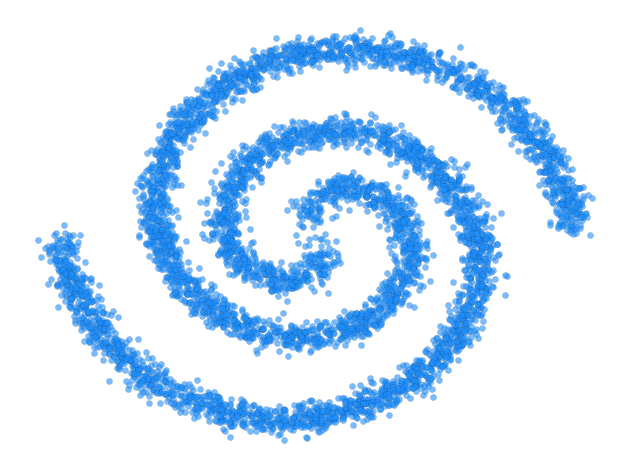
\includegraphics[width=\textwidth]{figures/spirals.png} 
        \caption{spirals}
    \end{subfigure}
    
    \vskip\baselineskip 
    \begin{subfigure}[b]{0.4\textwidth} 
        \centering
        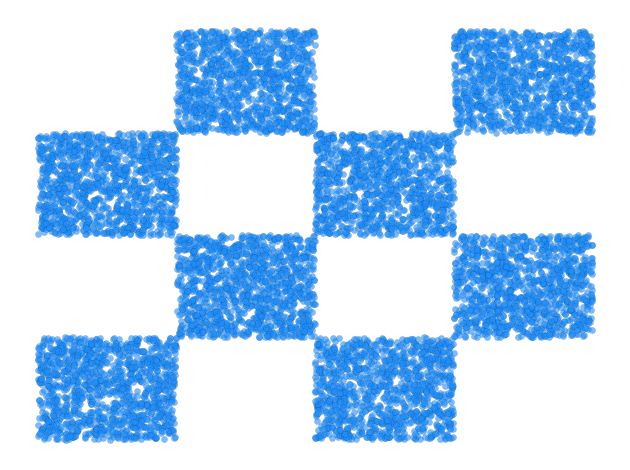
\includegraphics[width=\textwidth]{figures/board.png}
        \caption{board}
    \end{subfigure}
    
    \caption{Samples for all three datasets}
    \label{fig:2d_datasets}
\end{figure}


\subsection{Experiment 1}

In the basic first set of experiments we wanted to see the best possible results for each algorithm on each dataset. 

For each dataset we generated 20,000 datapoints and split them evenly for training and validation. However before the training process can start, recall 
that our model is governed by the learnable parameters $\boldsymbol \pi$ (mixture weights), $\boldsymbol \mu$ (means of components) and
$\boldsymbol \Sigma$ (covariance matrices of components) that need to be initialized in some manner and the hyperparameter $K$ (mixture count) that needs to be chosen. 

As for the learnable parameters, we initialized the mixture weights $\boldsymbol \pi$ uniformly 
\[
    \boldsymbol{\pi}_k = \frac{1}{K}, \quad k = 1, 2, \dots, K
\]
the covariance matrices $\boldsymbol \Sigma$ as identy matrices of size $D \times D$ 
\[
    \mathbf{\Sigma}_k = \mathbf{I}_D, \quad k = 1, 2, \dots, K
\]
where $D$ is the dimensionality of the data and the means $\boldsymbol \mu$ by computing cluster centers of the data with the sklearn \cite{sklearn} implementation of KMeans. 

As for $K$, trough some intitial testing we chose three different values, namely a minimal $K$, that is needed for producing reasonable results, 
a very large $K$ from which onward there are dimishing returns and a moderate $K$ in the middle between the minimal and the large $K$.

Now for the training process also recall that it is governed by the hyperparameters epochs (number of training iterations) for all algorithms and 
a learning rate (step-size for Gradient Descent) for all the gradient-based algorithms (GD, SM, SSM).
To choose these parameters we fixed $K$ to one of the three chosen values and did cross-validation by computing the validation set Log-Likelihood 
of the models with all possible remaining hyperparameter combinations and choosing the combination with the highest Log-Likelihood.

Results, more specifically Log-Likelihood, estimated densities and samples for all datasets and all values of $K$ with the best possible training-specific 
hyperparameters can be seen in the following three pages. Note that when setting the same random seed all of these results should be 
reproducable.

(I noticed that with higher Ks 40 and up SM and SSM didtn consistenly provide same results, maube becaus of autograd? EM and GD had 
always exact results .. not sure if i should include this)

\newpage
\begin{figure}[H]
    \centering
    \makebox[\textwidth][c]{\hspace*{-1cm} 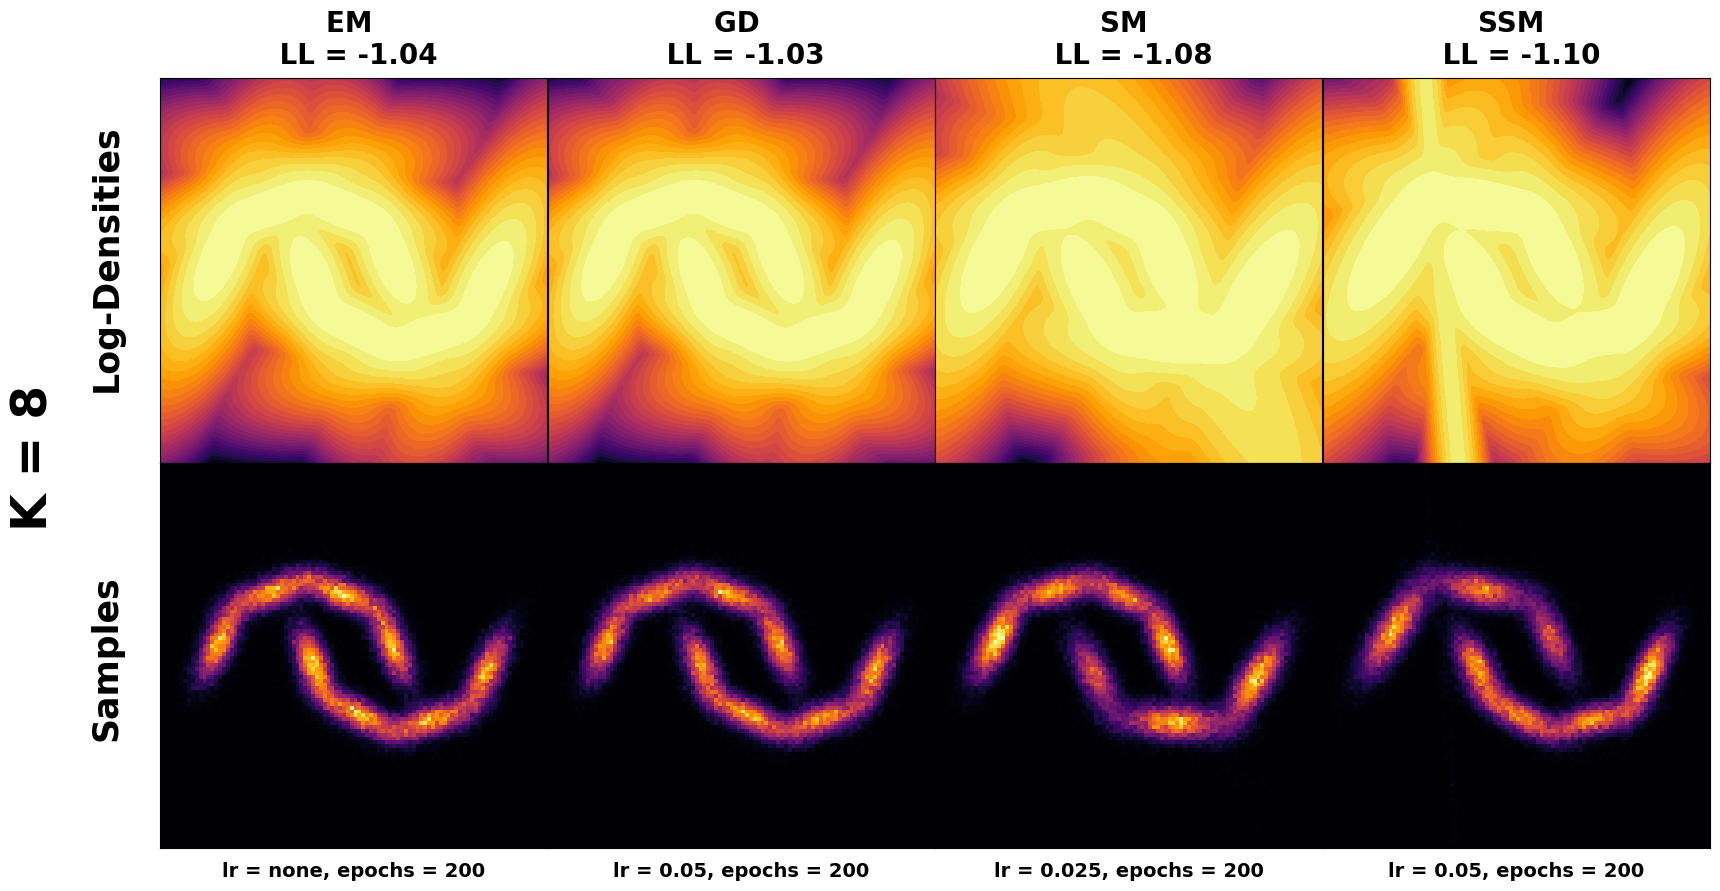
\includegraphics[width=0.9\textwidth]{figures/halfmoons/halfmoons_8.png}}
    \vskip 5pt
    \makebox[\textwidth][c]{\hspace*{-1cm} 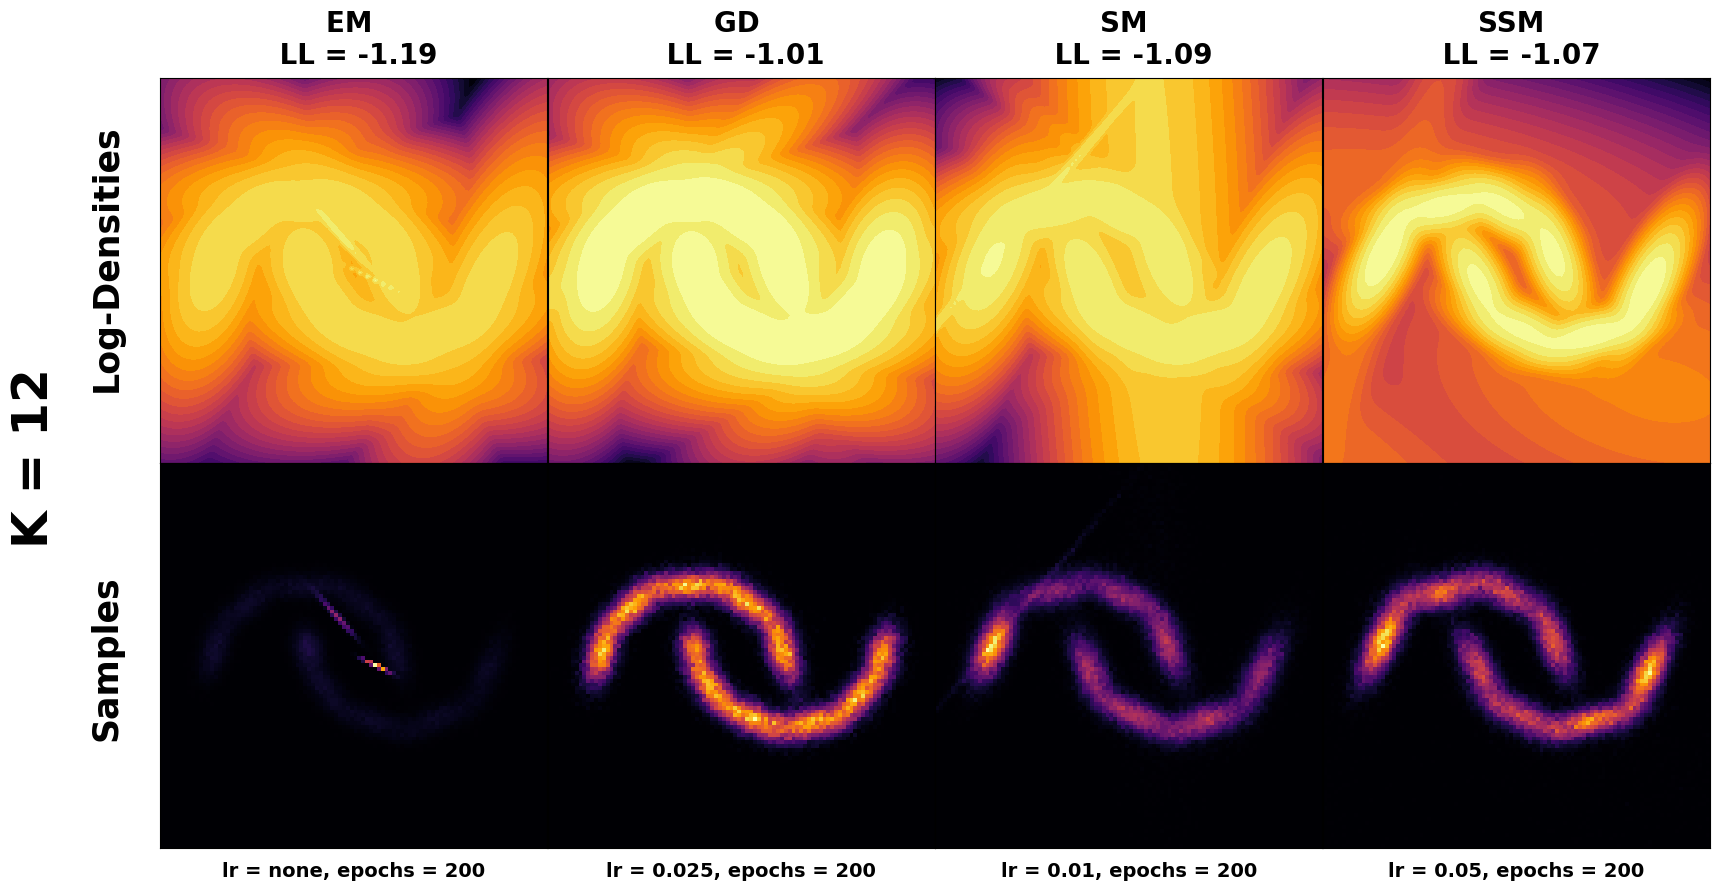
\includegraphics[width=0.9\textwidth]{figures/halfmoons/halfmoons_12.png}}
    \vskip 5pt
    \makebox[\textwidth][c]{\hspace*{-1cm} 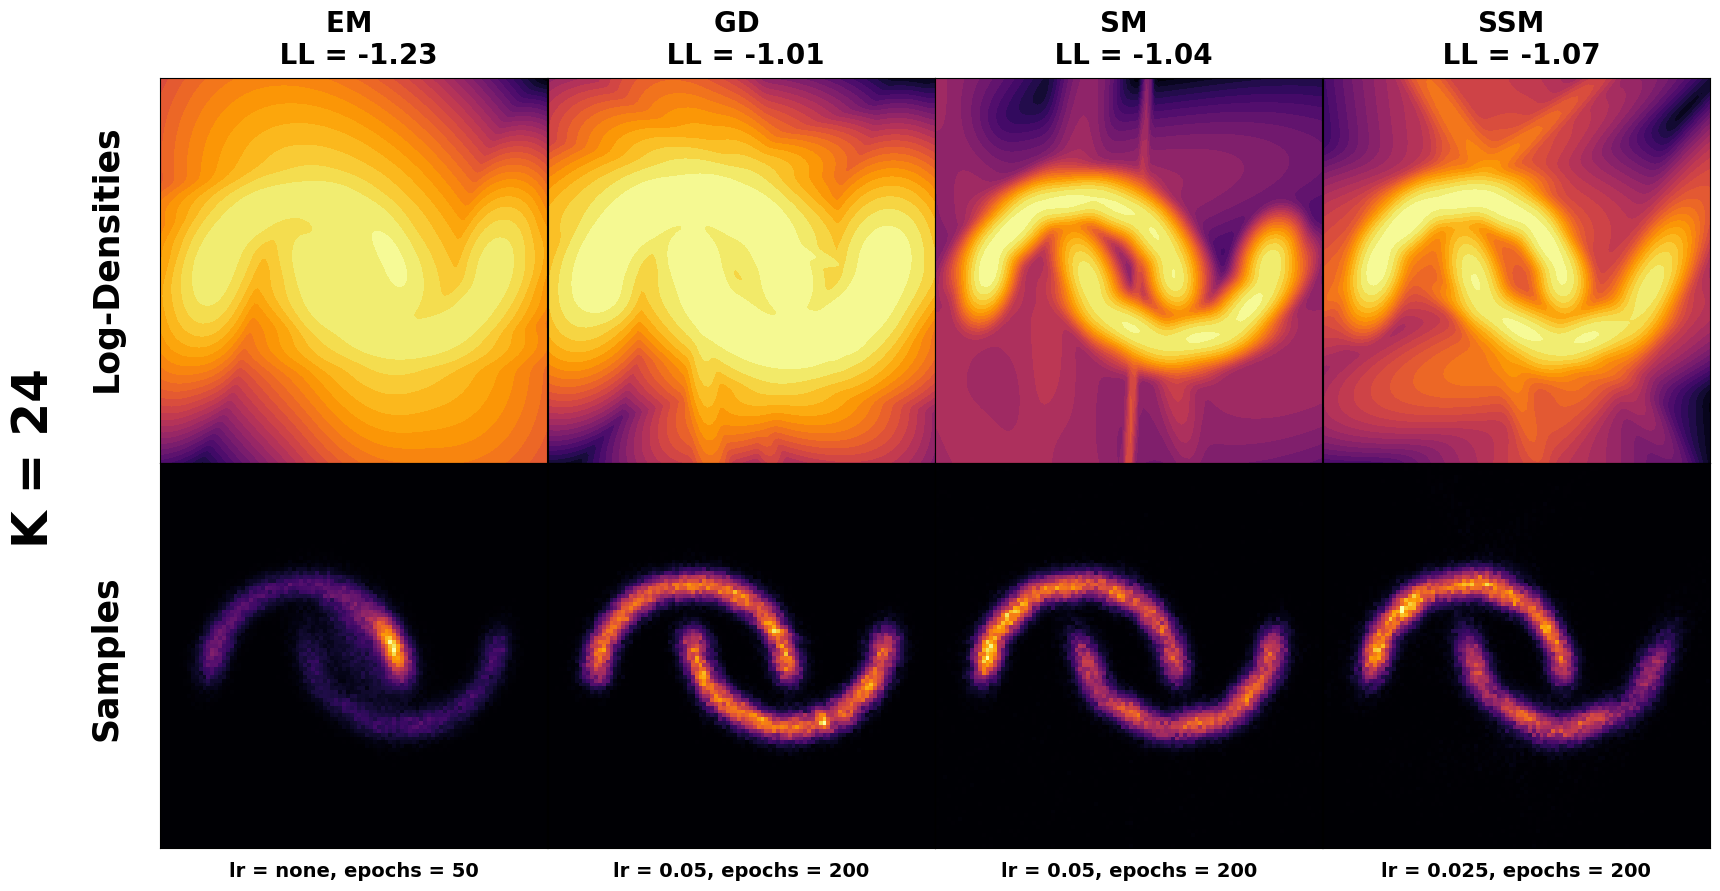
\includegraphics[width=0.9\textwidth]{figures/halfmoons/halfmoons_24.png}}
    \caption{Densities and Samples for the halfmoon dataset}
    \label{fig:exp_moons}
\end{figure}
\newpage
\begin{figure}[H]
    \centering
    \makebox[\textwidth][c]{\hspace*{-1cm} 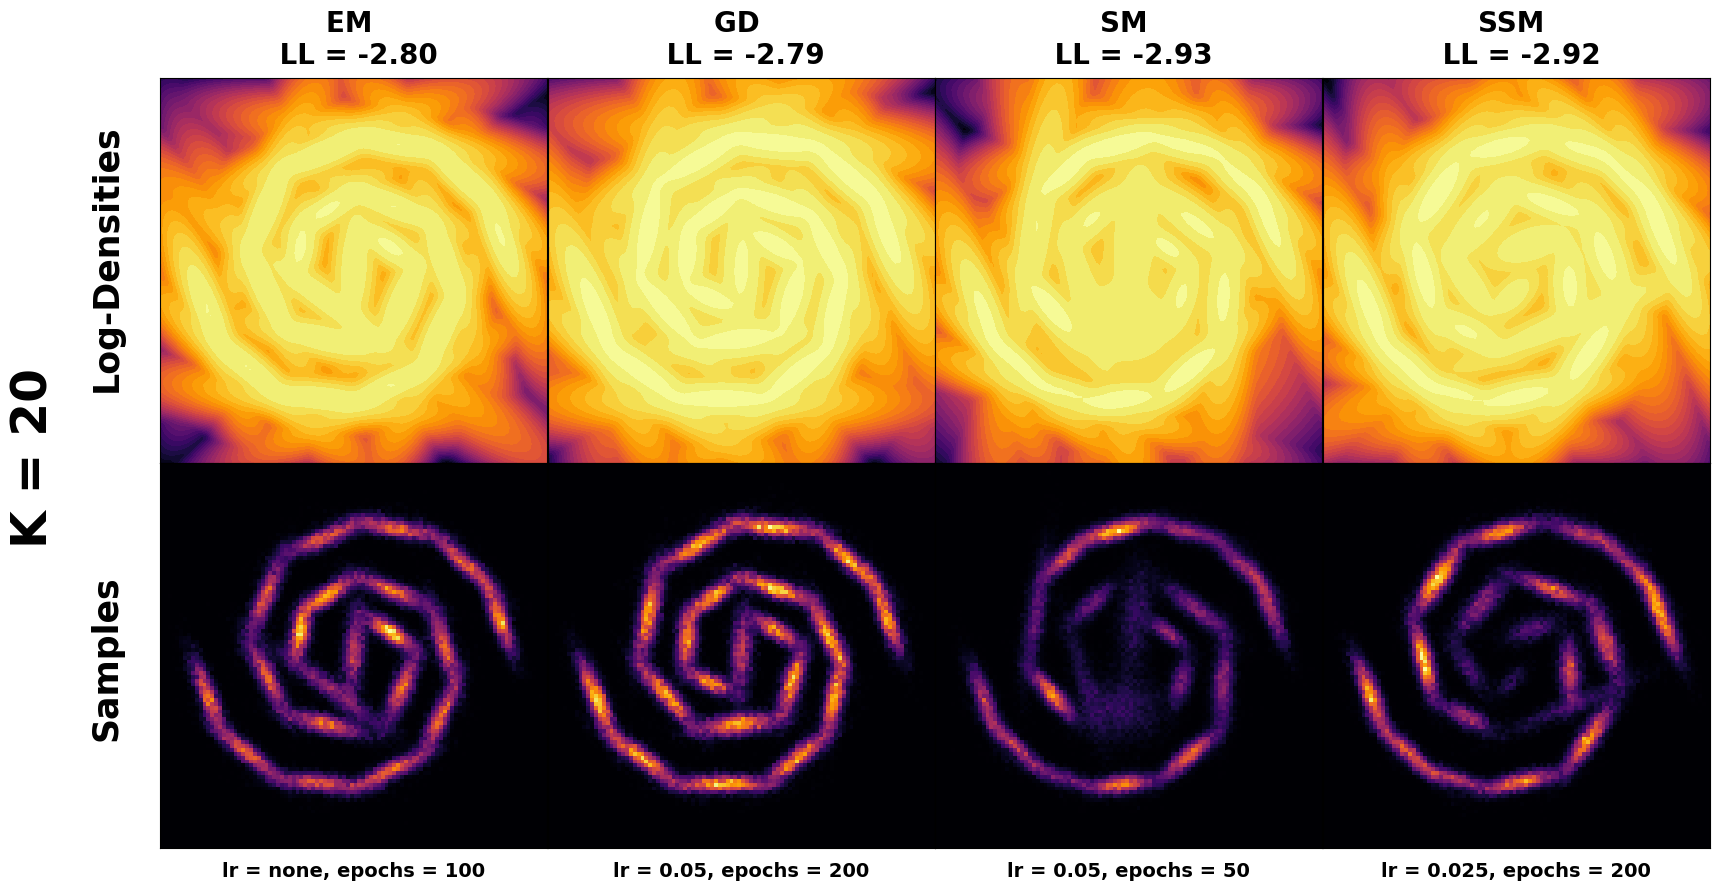
\includegraphics[width=0.9\textwidth]{figures/spirals/spirals_20.png}}
    \vskip 5pt
    \makebox[\textwidth][c]{\hspace*{-1cm} 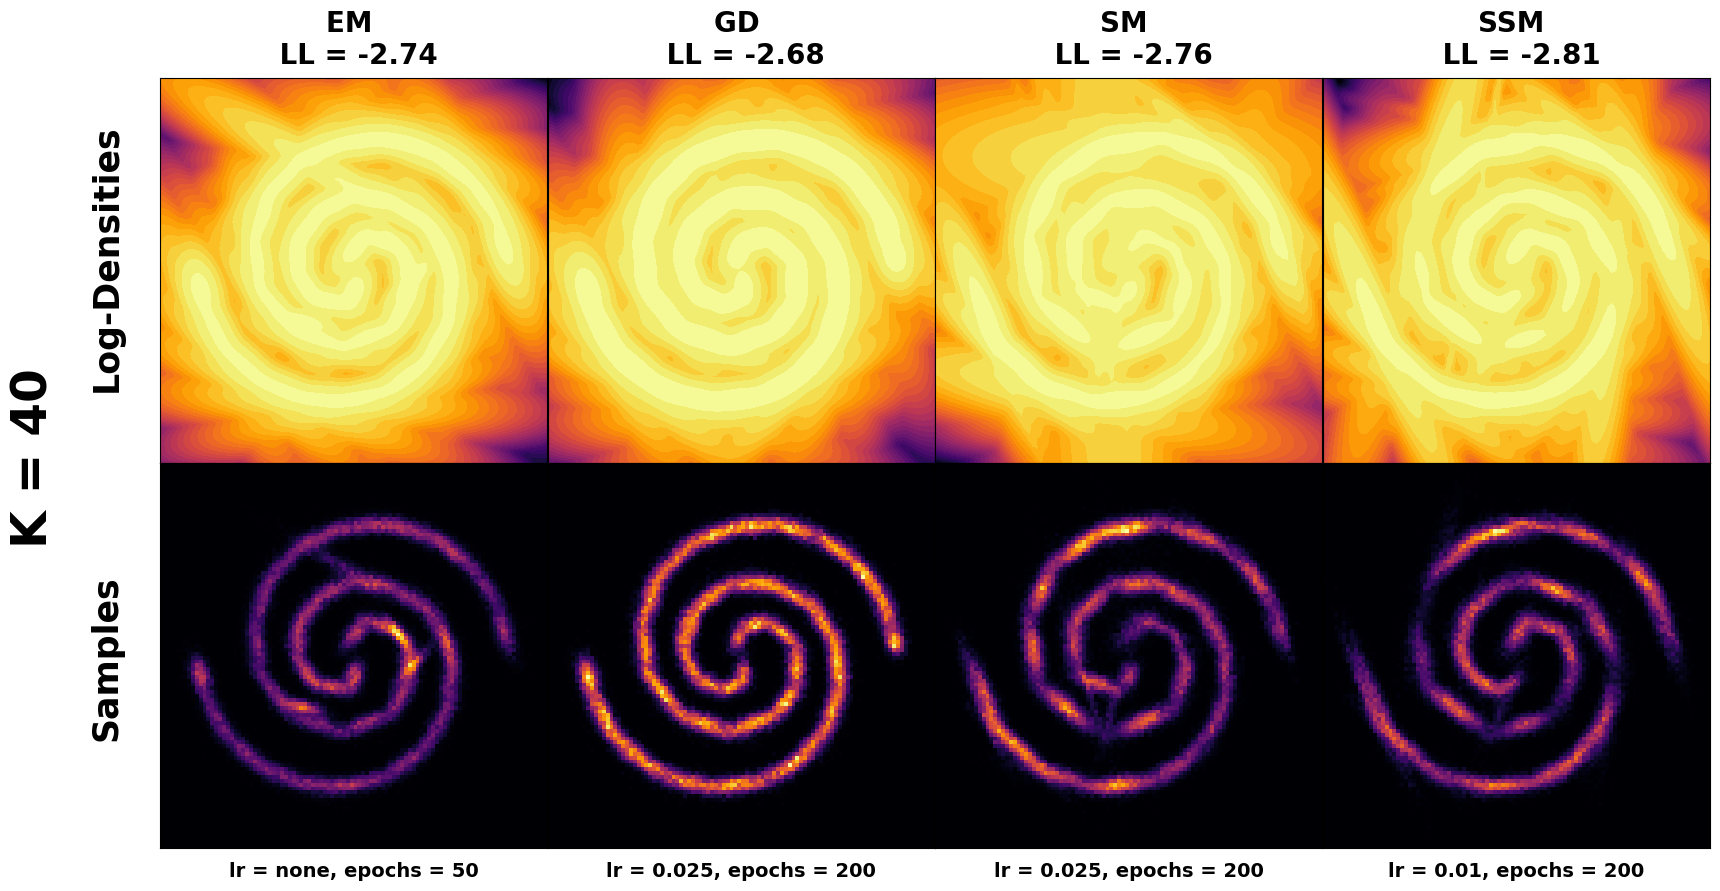
\includegraphics[width=0.9\textwidth]{figures/spirals/spirals_40.png}}
    \vskip 5pt
    \makebox[\textwidth][c]{\hspace*{-1cm} 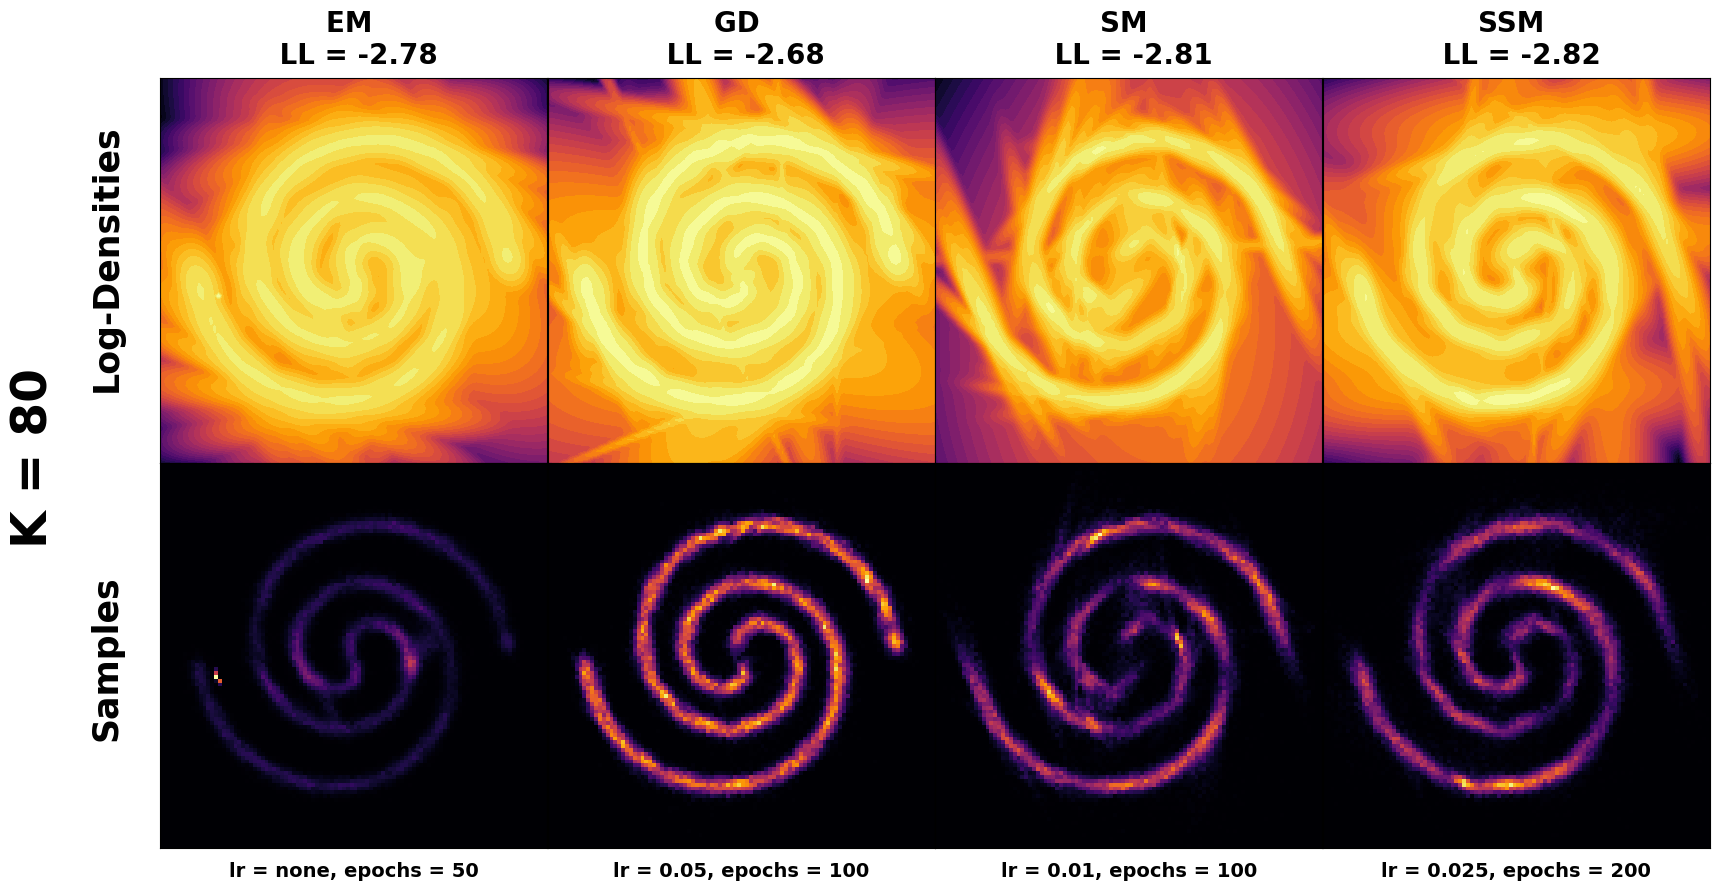
\includegraphics[width=0.9\textwidth]{figures/spirals/spirals_80.png}}
    \caption{Densities and Samples for the spirals dataset}
    \label{fig:exp_moons}
\end{figure}
\newpage
\begin{figure}[H]
    \centering
    \makebox[\textwidth][c]{\hspace*{-1cm} 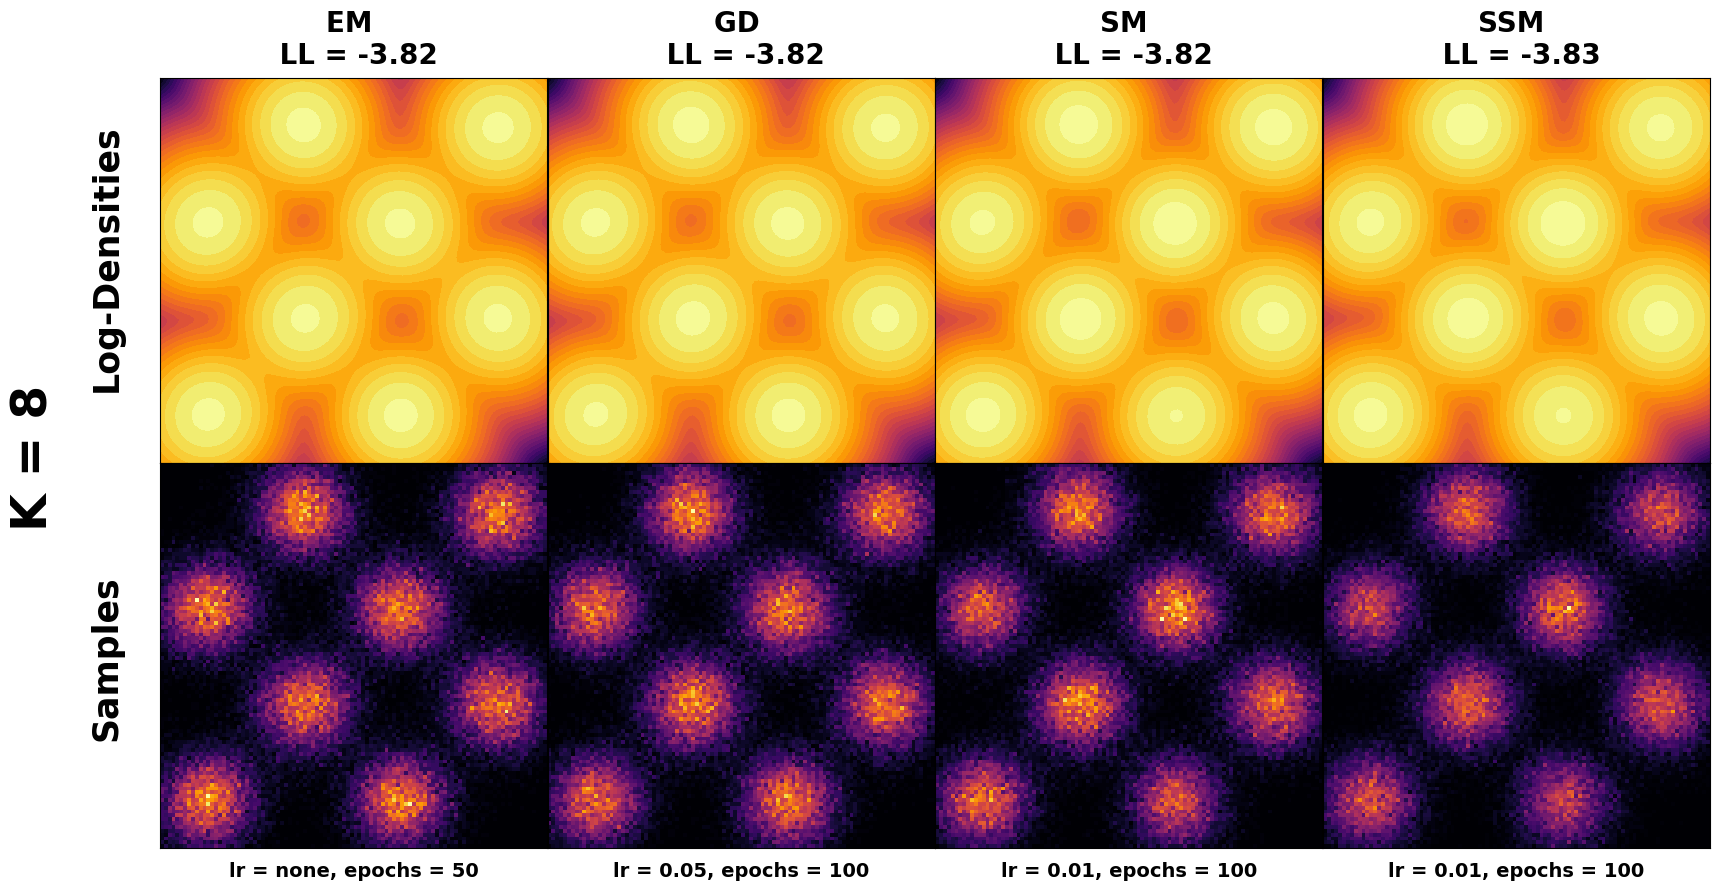
\includegraphics[width=0.9\textwidth]{figures/board_8.png}}
    \vskip 5pt
    \makebox[\textwidth][c]{\hspace*{-1cm} 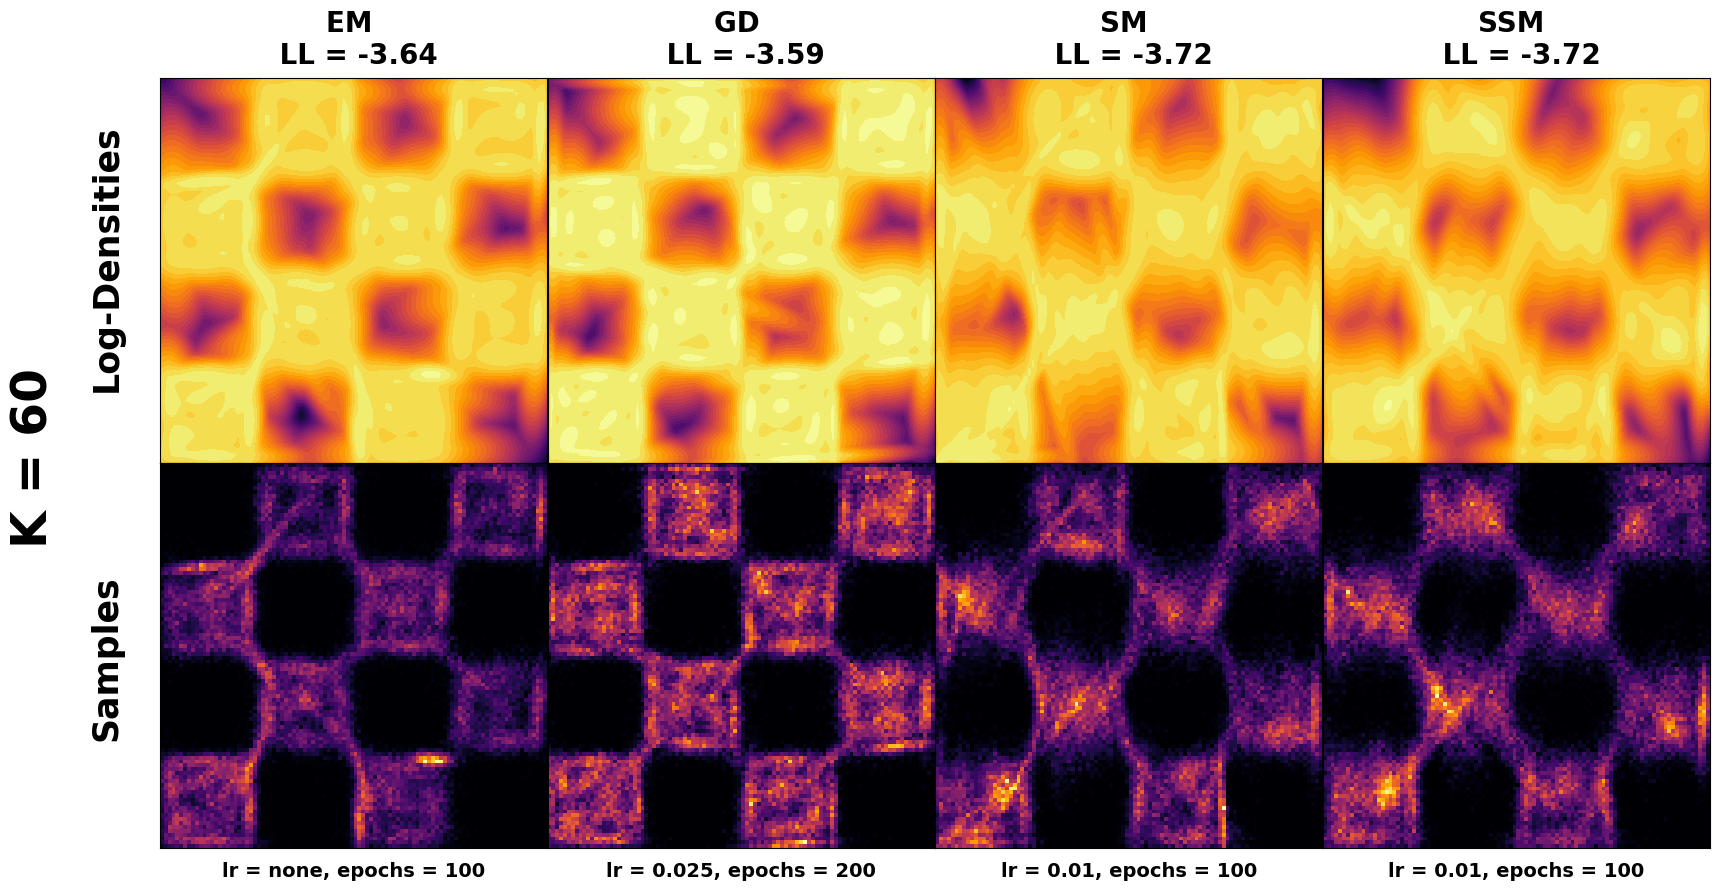
\includegraphics[width=0.9\textwidth]{figures/board_60.png}}
    \vskip 5pt
    \makebox[\textwidth][c]{\hspace*{-1cm} 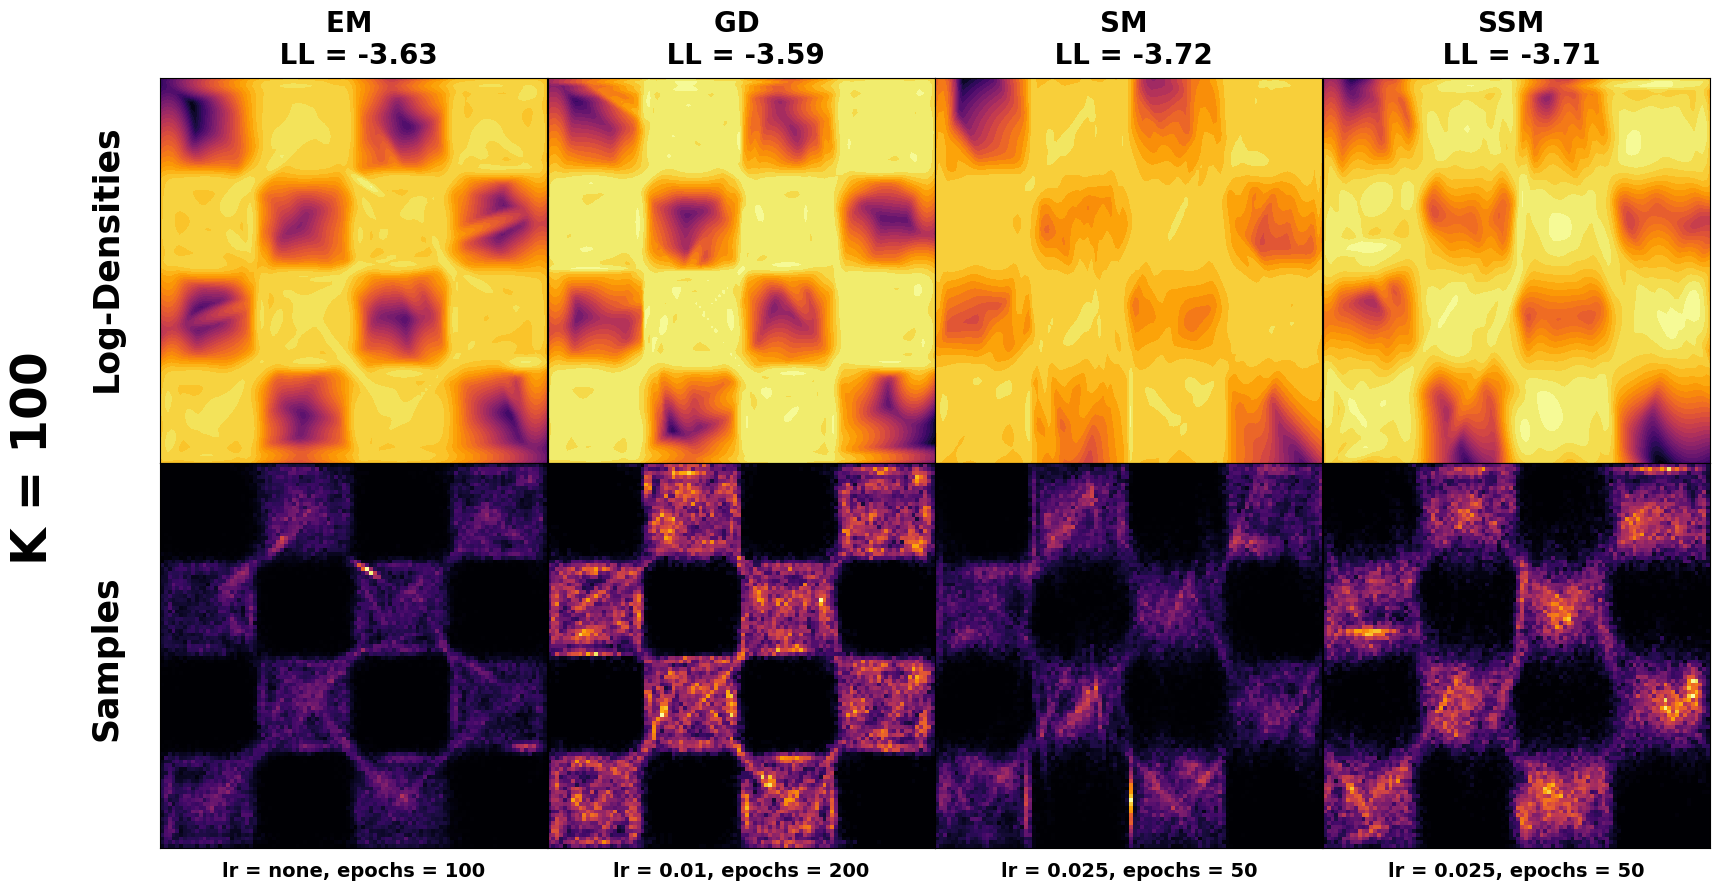
\includegraphics[width=0.9\textwidth]{figures/board_100.png}}
    \caption{Densities and Samples for the board dataset}
    \label{fig:exp_moons}
\end{figure}
\newpage

\subsection{Experiment 2}
\label{sec:2d_exp2}

To gain further insight in how the learning process differs for each algorithm we chose a dataset and a set of hyperparameters
where all algorithms perform somewhat similar and analized the Negative Log-Likelihood (NLL) over Training Iterations. 
Estimated density and samples and now also the mentioned training curve can be seen in Figure \ref{fig:halfmoons_10_logp}.

Note that because all algorithms except Sliced Score Matching are deterministic, we did multiple runs ($10$) for SSM and ploted the mean value 
with the standard deviation shaded. 

\begin{figure}[H]
    \centering
    \makebox[\textwidth][c]{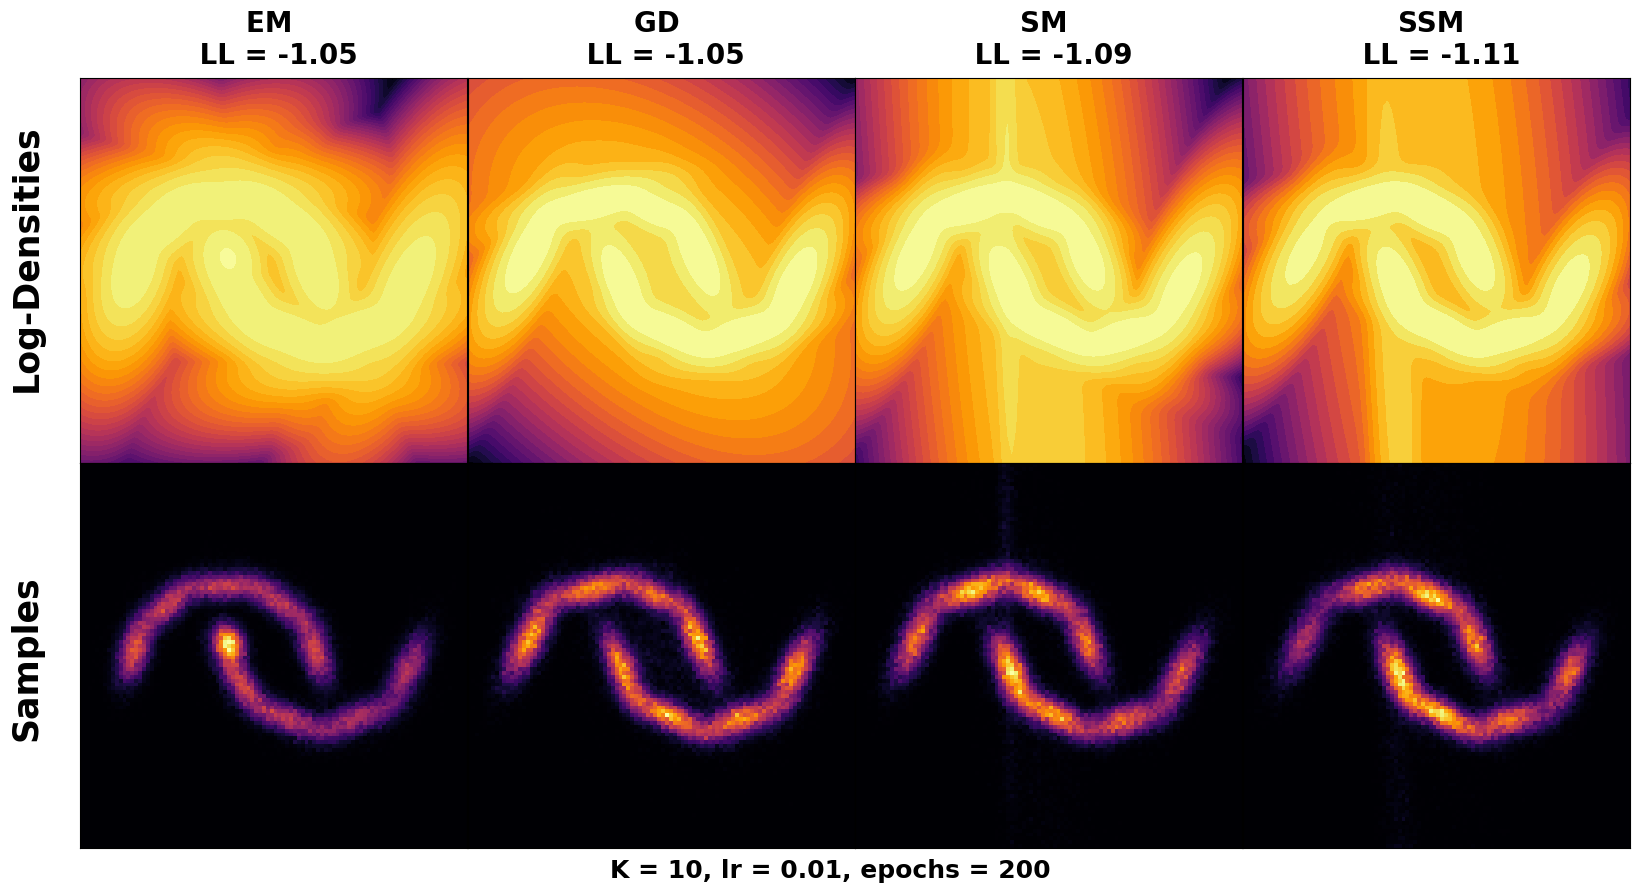
\includegraphics[width=0.6\textwidth]{figures/halfmoons/10_kmeans.png}}
    \makebox[\textwidth][c]{\hspace{-0.4cm} 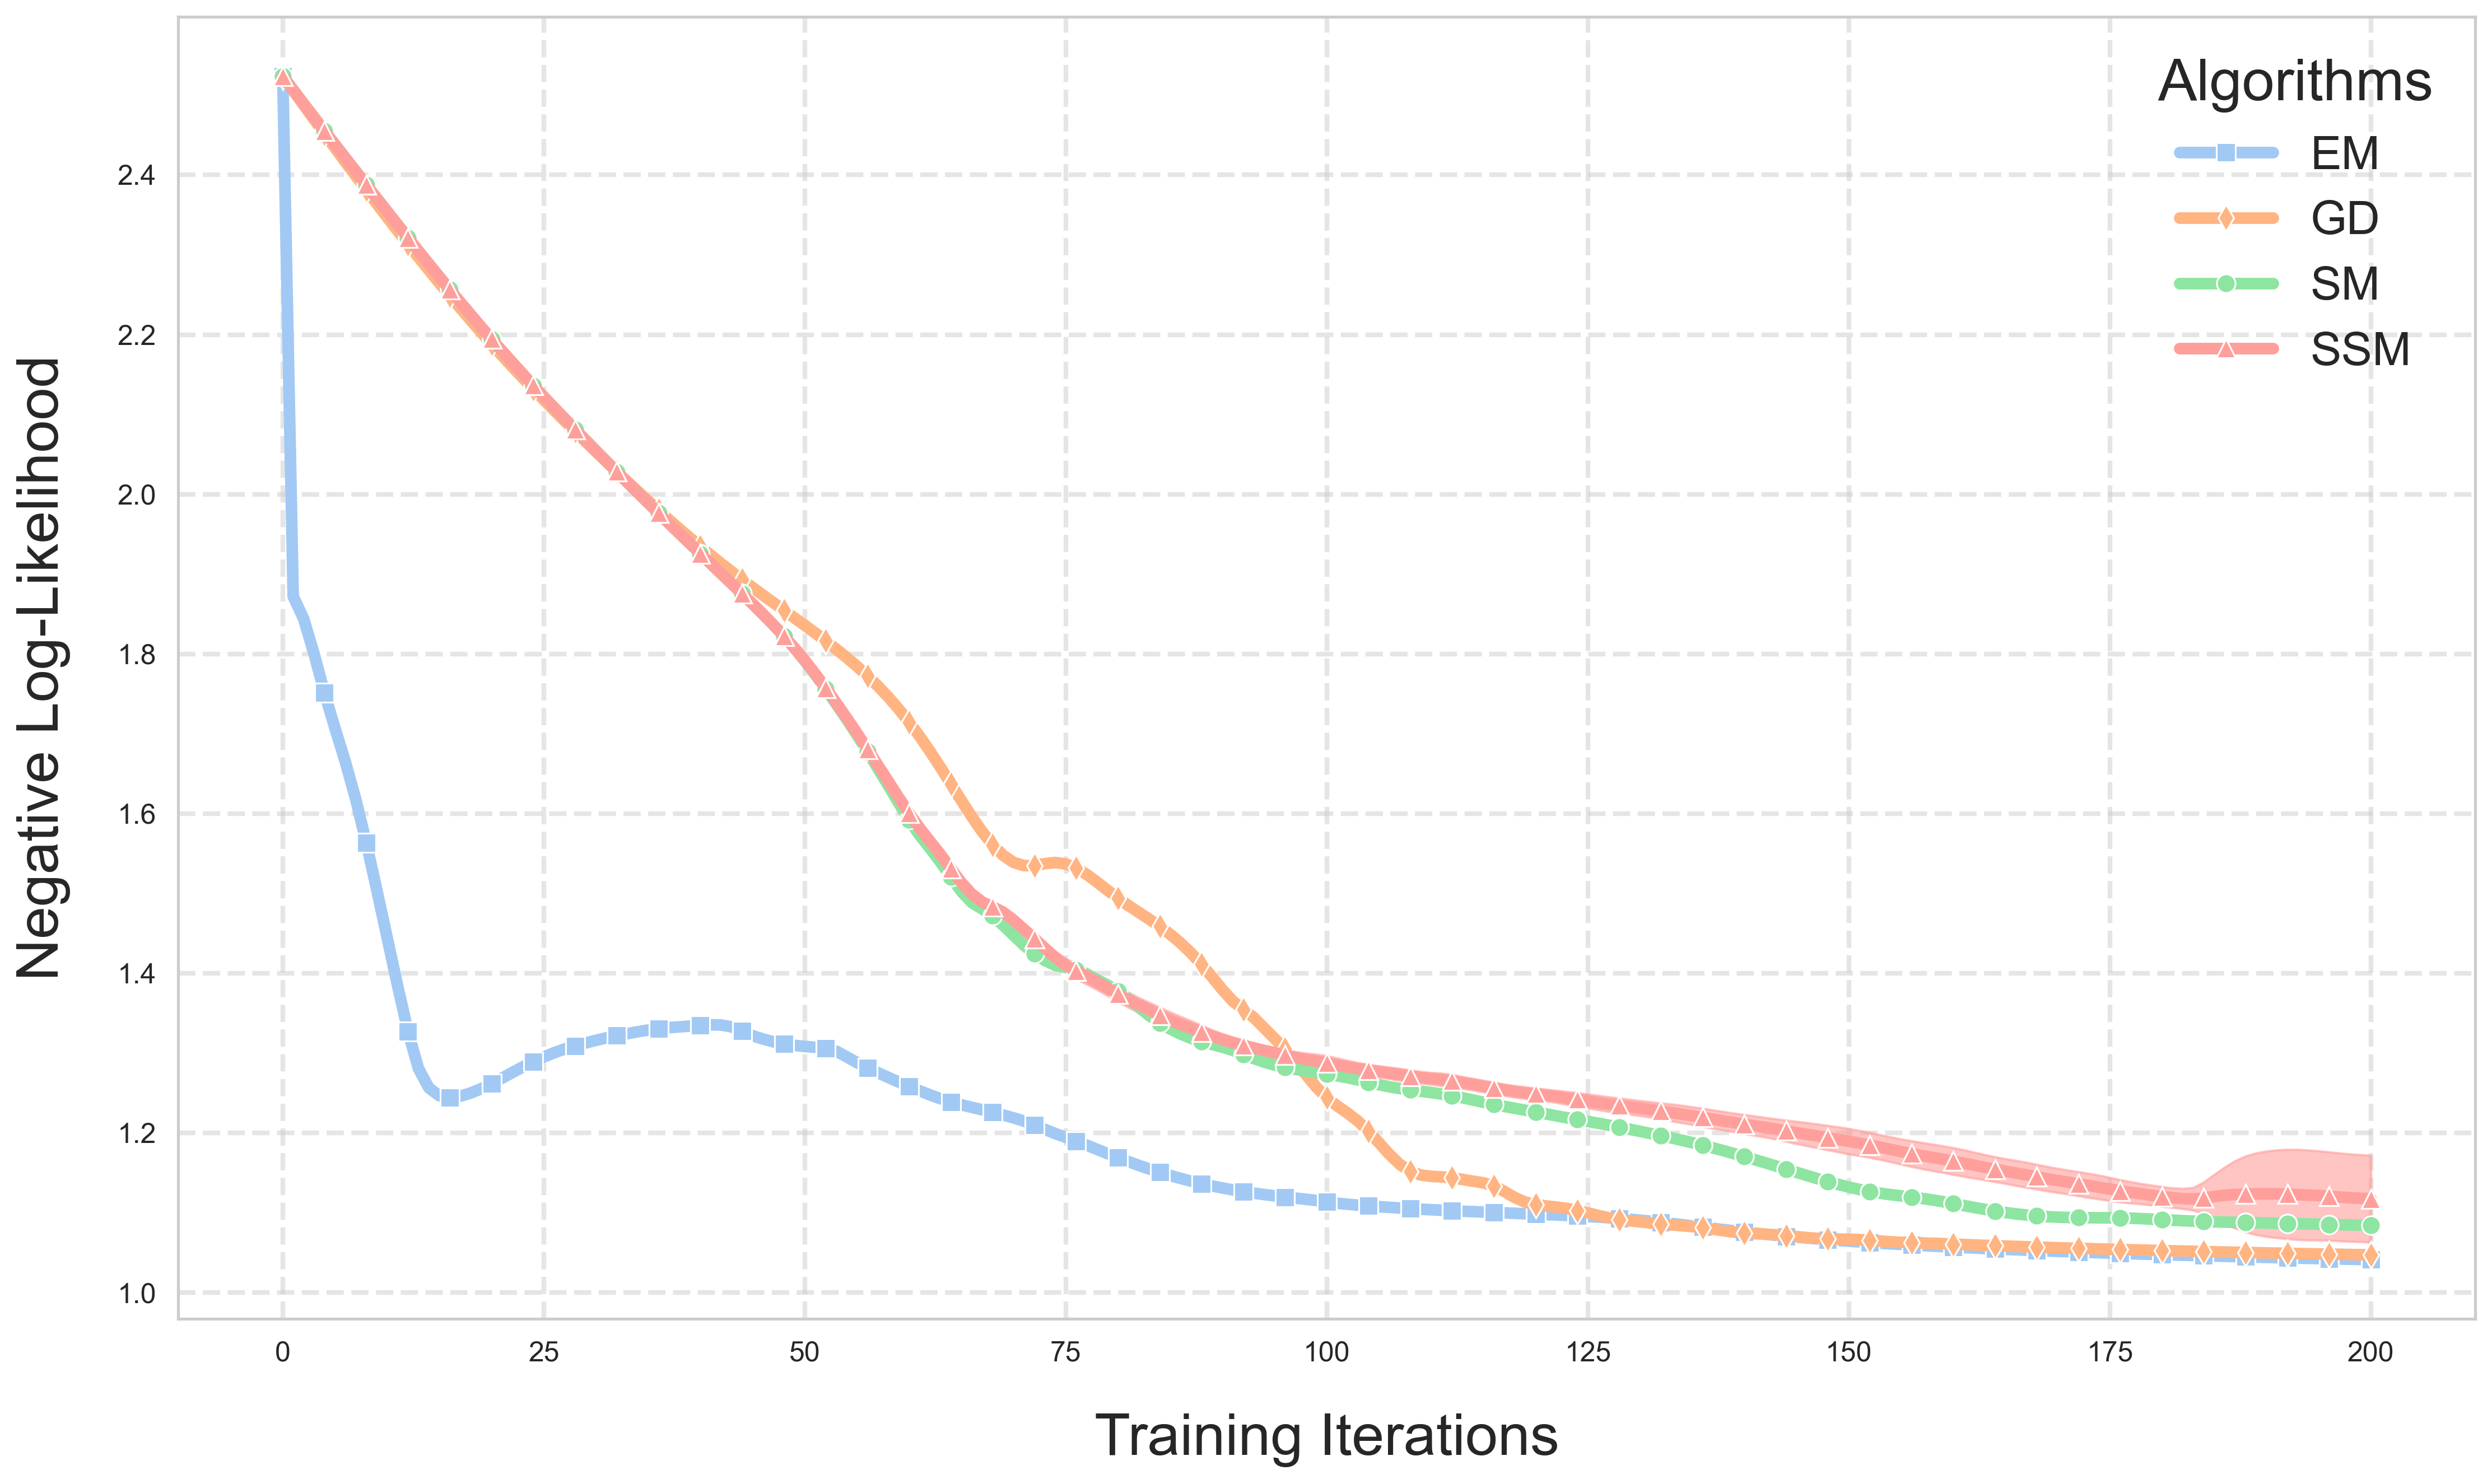
\includegraphics[width=0.8\textwidth]{figures/halfmoons/10_kmeans_logp.png}}
    \caption{Densities, Samples and NLL over Training Iterations}
    \label{fig:halfmoons_10_logp}
\end{figure}

On average SSM performs somewhere in the ballpark of SM but usually a little worse, which 
makes sense since SSM is only an approximation of SM. Sometimes the stochastic nature of SSM can also 
by luck perform better than SM but this is only happens very rarely. 

\subsection{Experiment 3}
\label{sec:2d_exp3}

Another point we wanted to examine was the initialization of the learnable parameters.
With our data it is quite straightforward to initialize the means, which up to now has been done with KMeans, but this is not always the case.
Also initializing the weights uniformly convieniently makes a lot of sense with our data, however the initialization of both of these 
learnable parameters can be problematic and a lot of times this has to be done randomly. Therefore we also analized how each algorithm 
behaves when these parameters are initialized randomly. To intitialize the means we draw $K$ random datapoints from our training data and 
to initialize the weights we just draw random numbers from $0$ to $1$ and normalize them so they sum to one.

In Figure \ref{fig:halfmoons_10_random_logp} the mean Log-Likelihood and standard deviation over $10$ runs with random initialization in each run can be seen. 
On this simple dataset it appears that random initialization performs relatively similar to the KMeans initialization when comparing 
to the NLL over Epochs curve from Figure \ref{fig:halfmoons_10_logp}. For some concrete results (Densities and Samples) refer to the Appendix.

\begin{figure}[H]
    \centering
    \makebox[\textwidth][c]{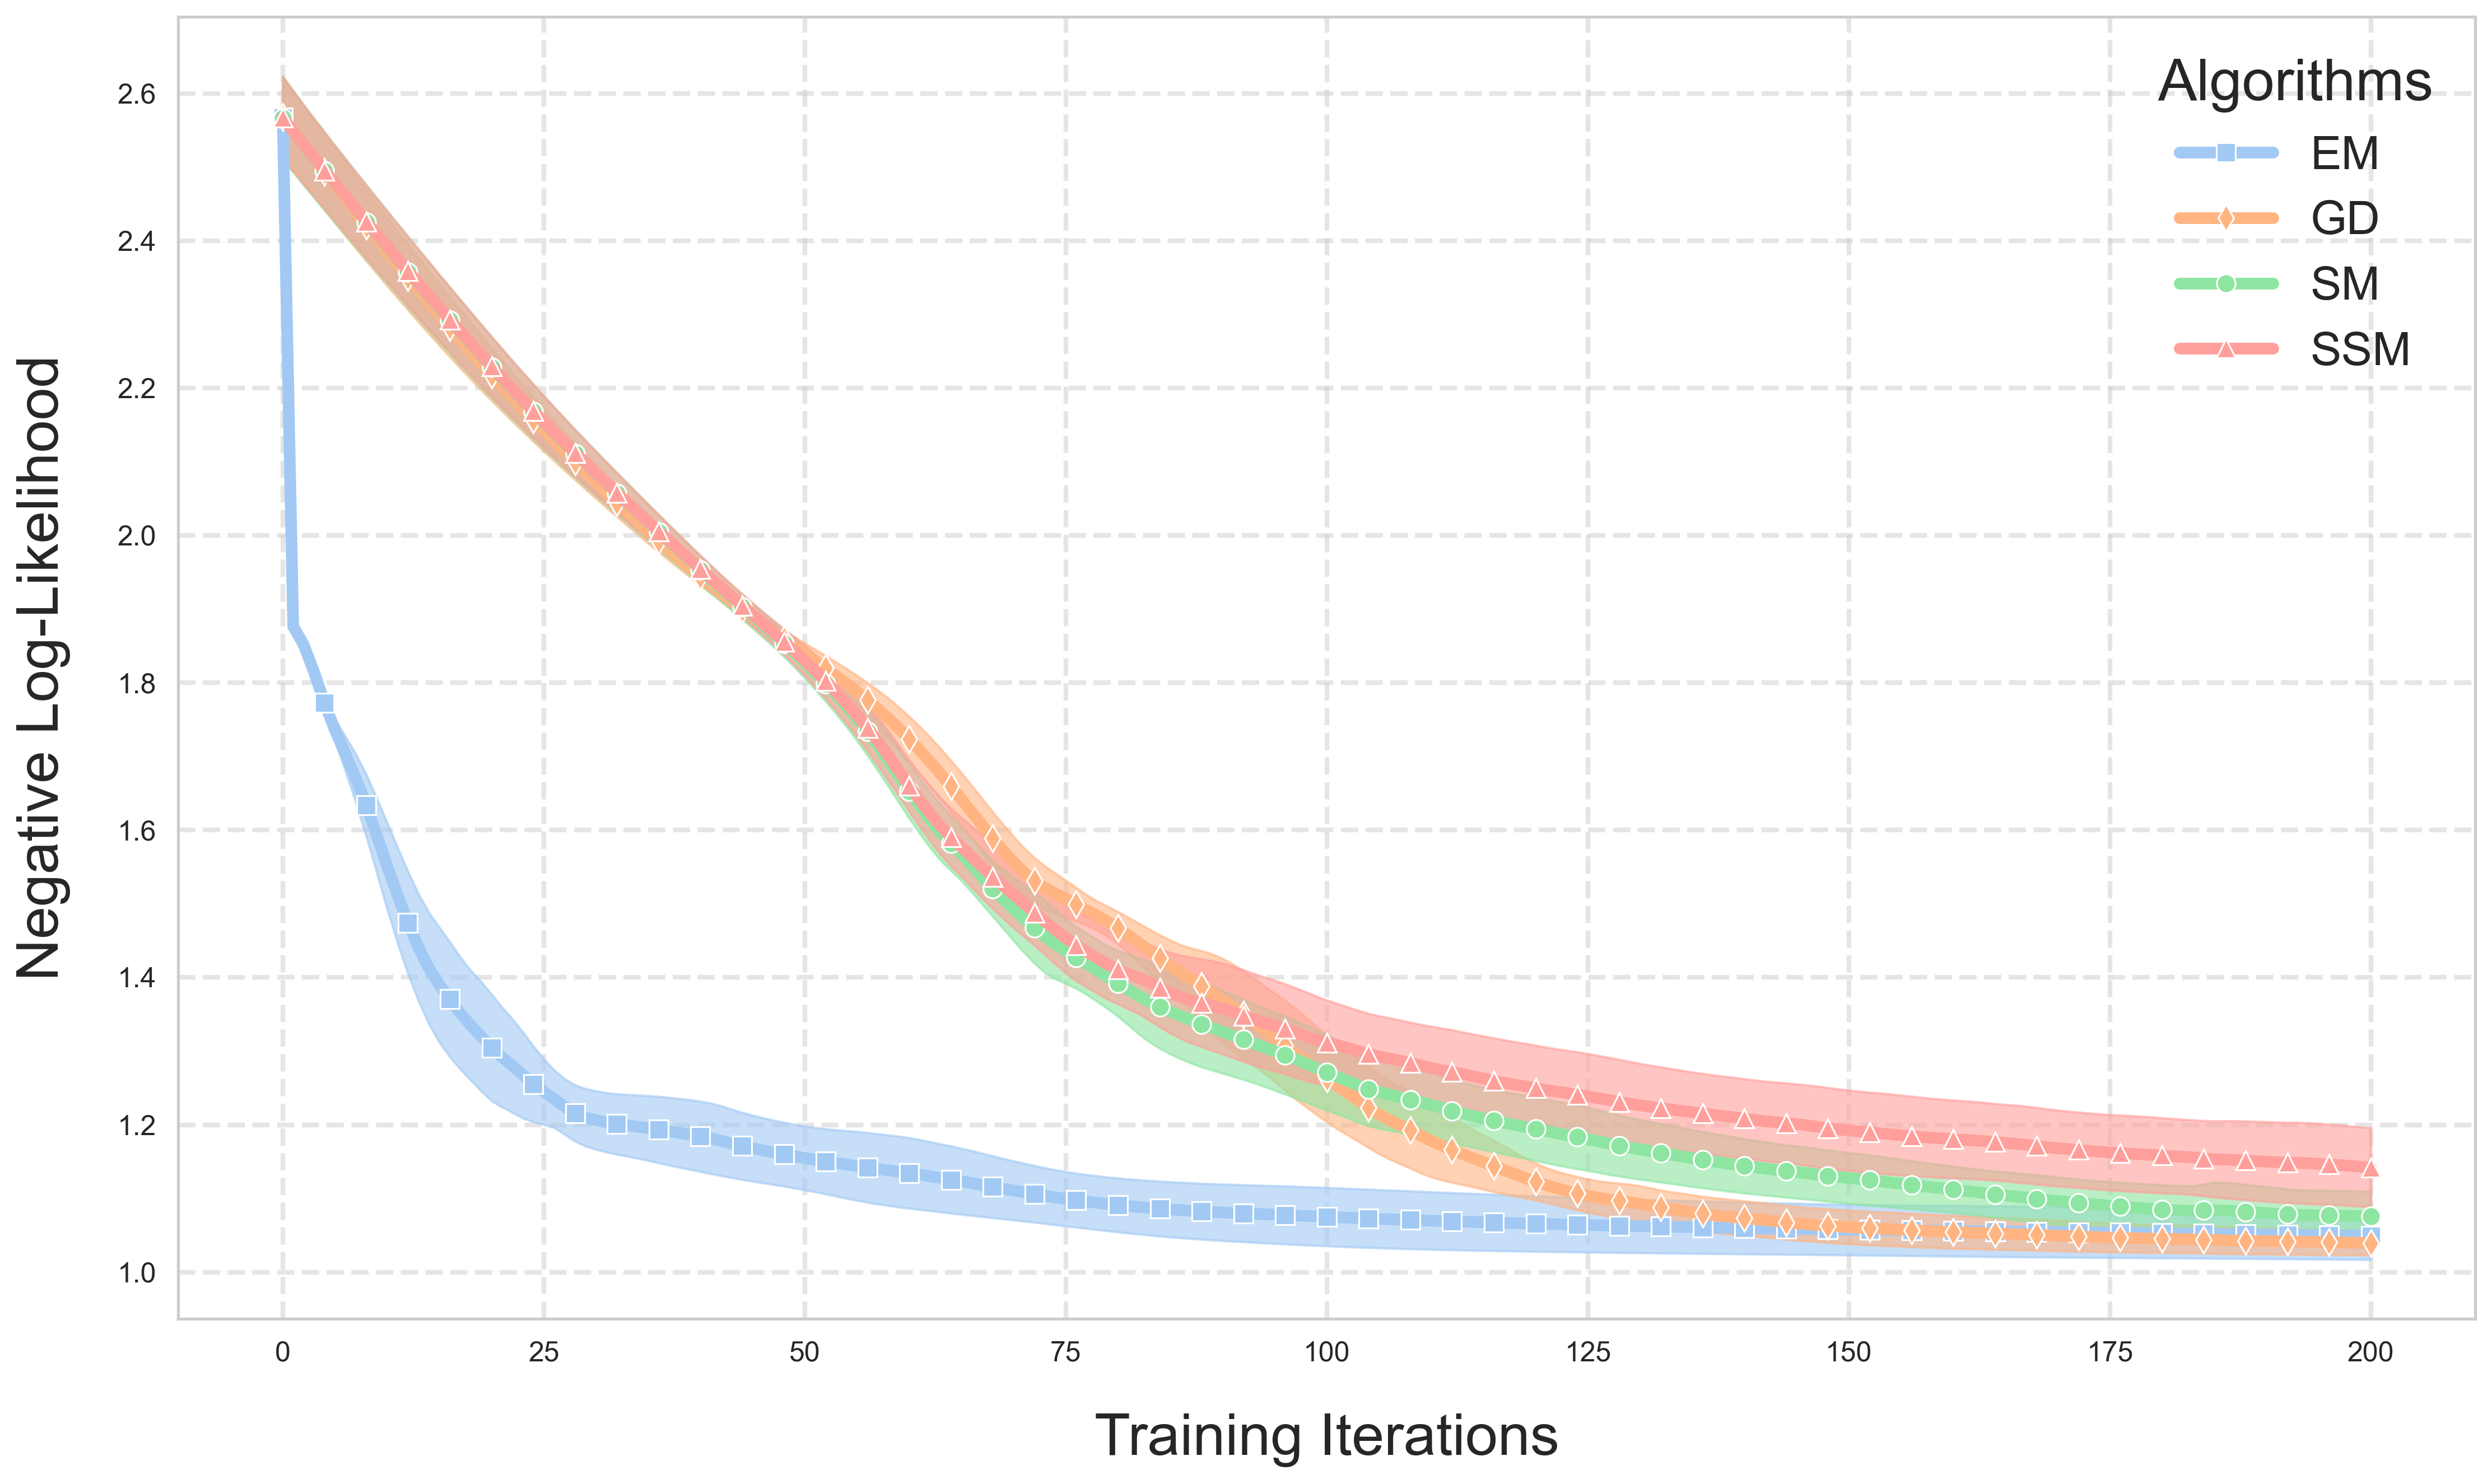
\includegraphics[width=0.9\textwidth]{figures/halfmoons/10_random_logp.png}}
    \caption{Negative Log Likelihood over Epochs with random parameter initialization}
    \label{fig:halfmoons_10_random_logp}
\end{figure}

We repeated this Experiment for a more complex dataset where all algorithms performed somewhat worse to 
when doing KMeans initialization but overall the difference between the algorithms, in which we are mostly intrested, 
remained basically the same. For those interested these results can also be found in the Appendix.

\subsection{Experiment 4}

Before continuing with the high dimensional experiments, we wanted to compare SSM and SM more extensively since in the high dimensional case
only SSM is usable. 

\newpage
\section{Images Density Estimation}

I used the MNIST Dataset \cite{mnist} 

\begin{figure}[H]
    \centering
    % First subfigure
    \begin{subfigure}[b]{0.3\textwidth}
        \centering
        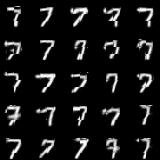
\includegraphics[width=\textwidth]{figures/mnist_EM.png} % replace with your image file
        \caption{EM}
        \label{fig:sub1}
    \end{subfigure}
    \hfill
    % Second subfigure
    \begin{subfigure}[b]{0.3\textwidth}
        \centering
        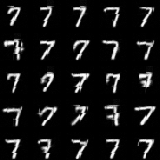
\includegraphics[width=\textwidth]{figures/mnist_SGD.png} % replace with your image file
        \caption{SGD}
        \label{fig:sub2}
    \end{subfigure}
    \hfill
    % Third subfigure
    \begin{subfigure}[b]{0.3\textwidth}
        \centering
        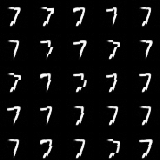
\includegraphics[width=\textwidth]{figures/mnist_SSM.png} % replace with your image file
        \caption{SSM}
        \label{fig:sub3}
    \end{subfigure}

    \caption{MNIST Samples}
    \label{fig:three_images}
\end{figure}